\chapter{Physical Space, Time, and Dimensional Analysis}
\label{ch:foundations}

\begin{chapterintro}
\textbf{Chapter Objectives:} In this opening chapter, we establish the foundational ontology of classical mechanics. You will master the SI metric standard; formulate rigorous dimensional equations; apply the Buckingham $\Pi$ theorem to discover physical scaling laws without solving differential equations; and develop intuitive order-of-magnitude estimation skills essential for theoretical and experimental physics.
\end{chapterintro}

\section{The Physical Framework of Classical Mechanics}

Classical point mechanics models the physical universe as a collection of idealized particles moving through a continuous, three-dimensional Euclidean space $\mathbb{R}^3$ parametrized by an absolute, uniformly flowing time parameter $t \in \mathbb{R}$.

\begin{definitionbox}{The Material Point (Classical Particle)}
A \textbf{material point} (or \emph{point particle}) is an idealized mathematical body whose spatial dimensions are negligible compared to the characteristic geometric scales of its trajectory and environment, but which nevertheless possesses a finite non-zero inertial mass $m > 0$.
\end{definitionbox}

Whether an object can be treated as a point particle depends not on its intrinsic size, but on the \textbf{scale of the physical phenomenon} under study:
\begin{itemize}[leftmargin=1.4em,itemsep=3pt]
  \item The Earth has a mean diameter of $12\,742\ \mathrm{km}$, yet when computing its orbital trajectory around the Sun (orbital radius $R \approx 1.50\times 10^8\ \mathrm{km}$), its diameter represents less than $0.008\%$ of the orbital span; treating Earth as a material point yields predictions accurate to parts in a million.
  \item Conversely, when studying the precession of the equinoxes, oceanic tidal bulges, or atmospheric circulation, the finite extension and non-spherical mass distribution of Earth are central, requiring rigid body and continuum mechanics.
\end{itemize}

\begin{historicalbox}{Galileo Galilei and the Mathematical Language of Nature}
\begin{minipage}{0.28\textwidth}
\centering
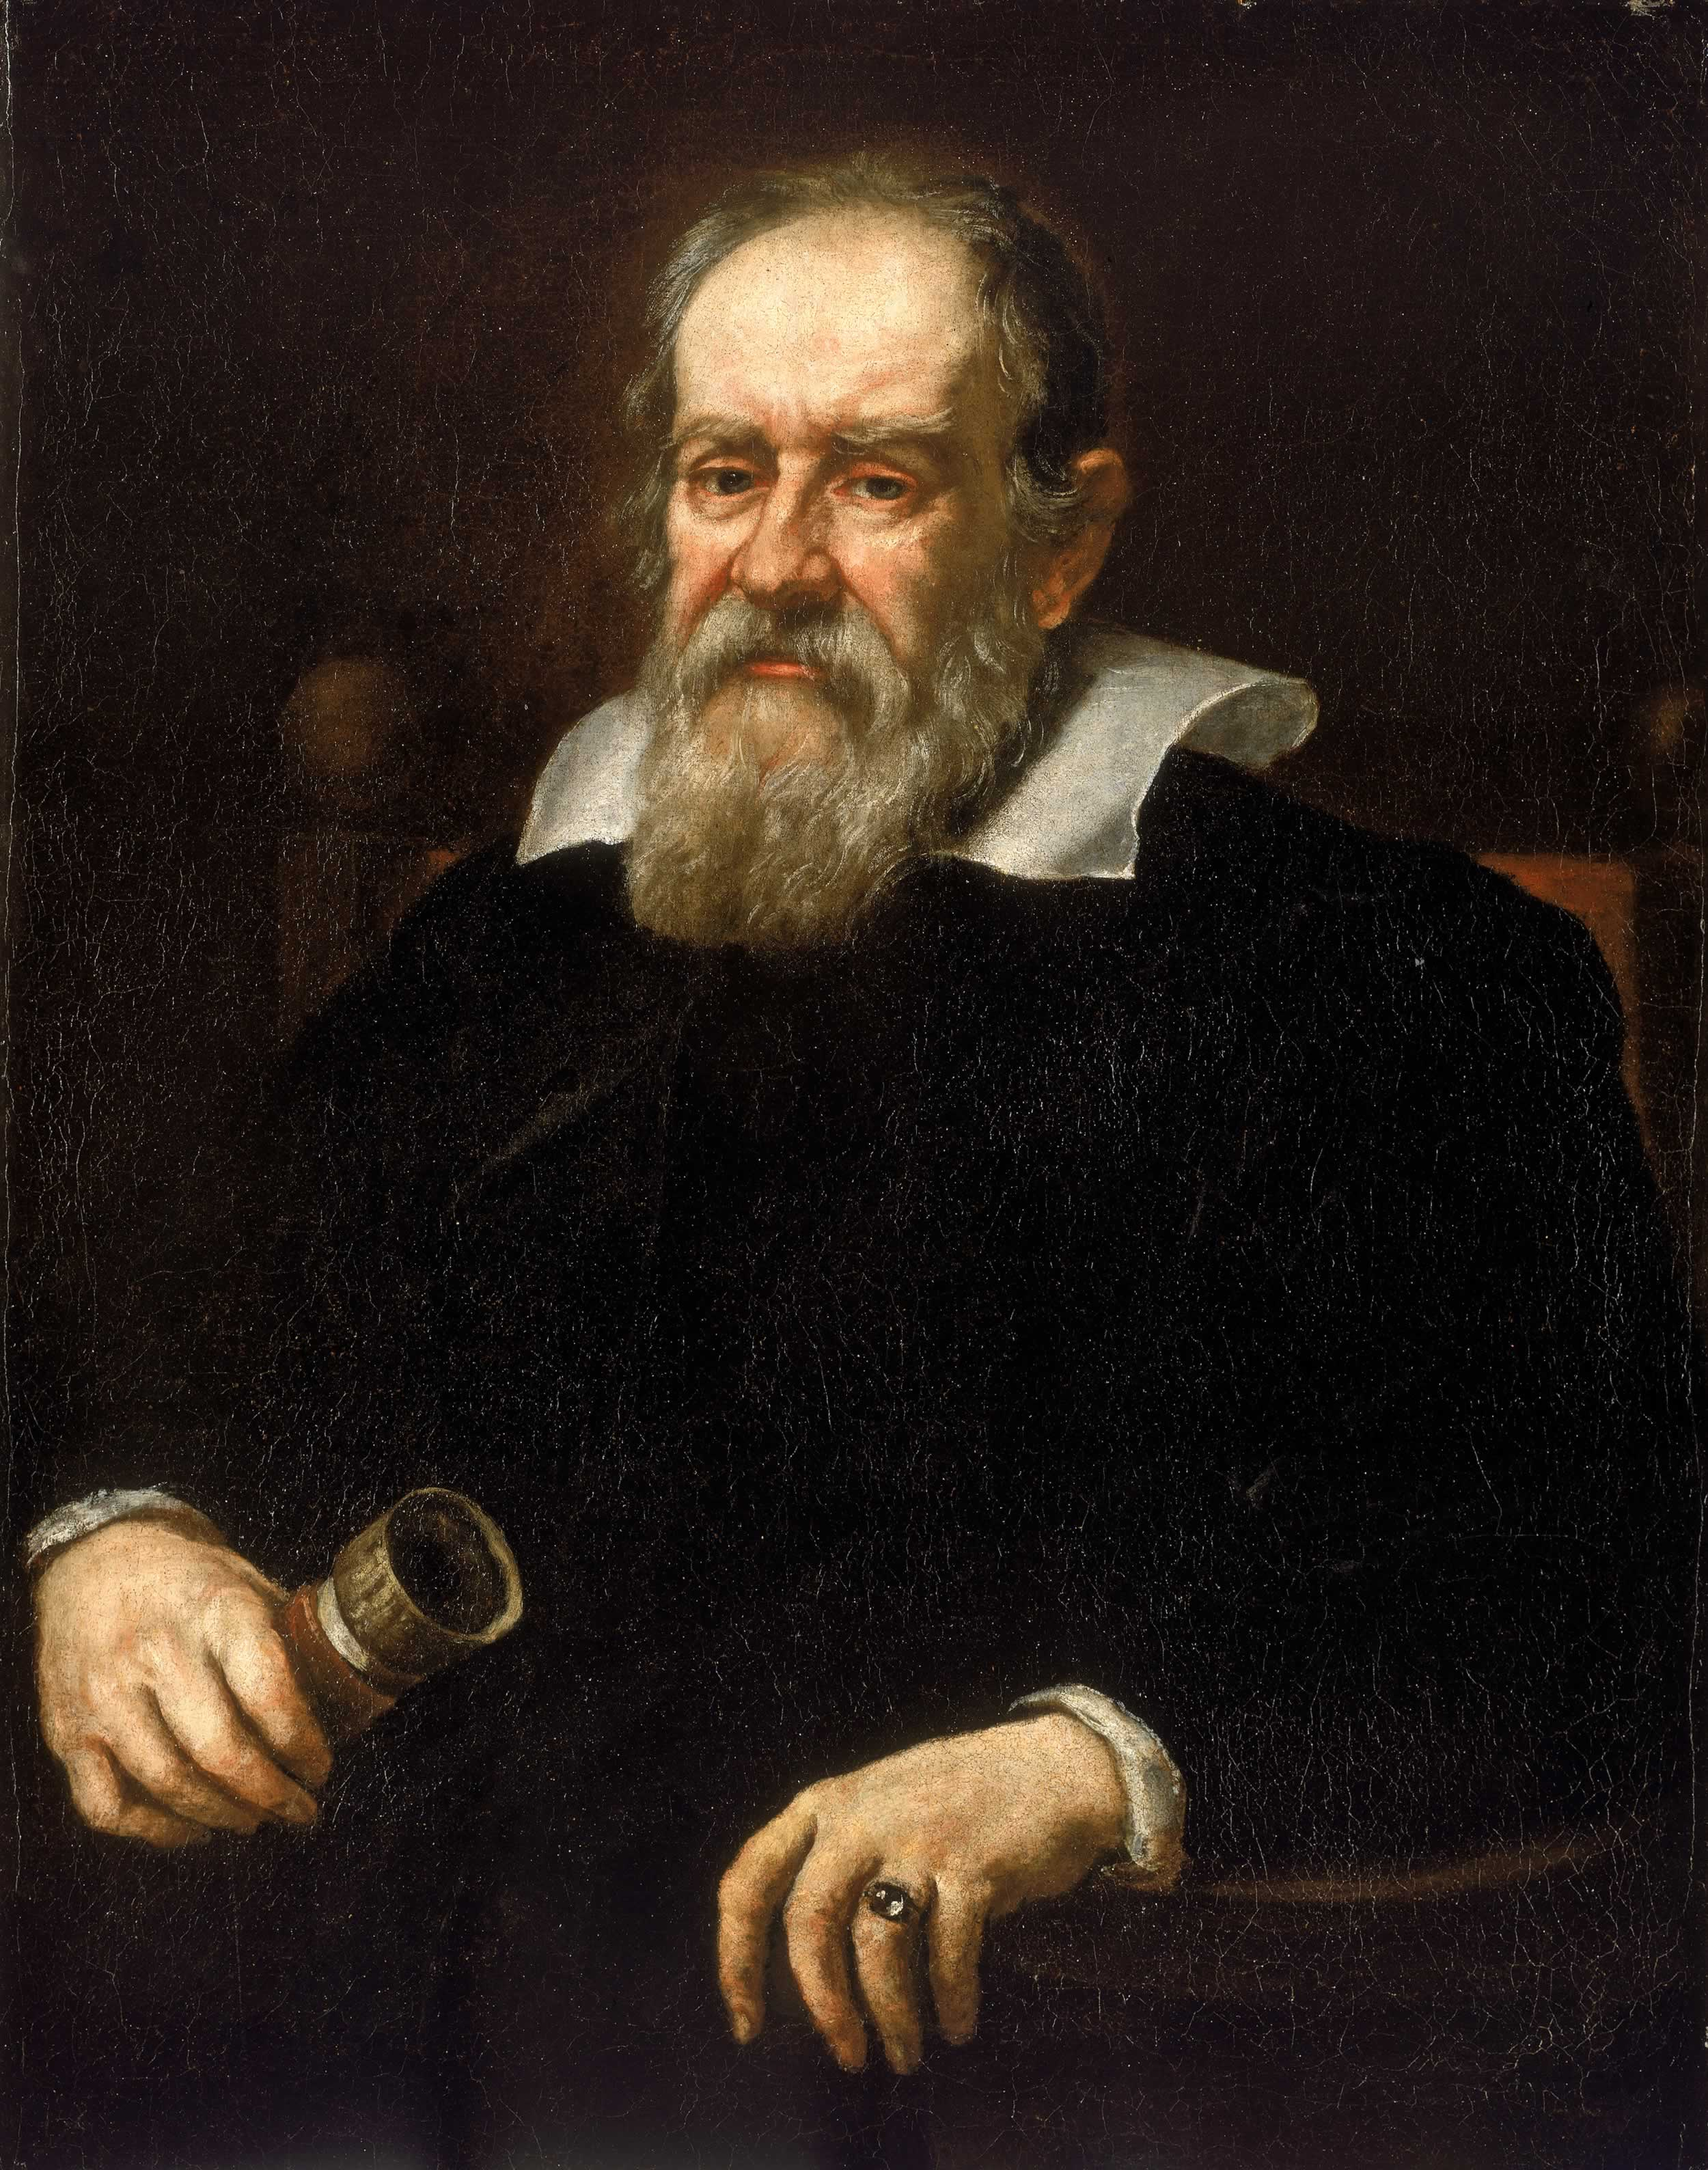
\includegraphics[width=0.95\textwidth]{images/galileo.jpg}
\captionof{figure}{Galileo Galilei (1564--1642), portrait by Justus Sustermans (1636, Uffizi Gallery).}
\end{minipage}\hfill
\begin{minipage}{0.68\textwidth}
In his 1623 treatise \emph{Il Saggiatore} (The Assayer), Galileo Galilei declared that the grand book of the universe ``cannot be understood unless one first learns to comprehend the language and read the letters in which it is composed. It is written in the language of mathematics, and its characters are triangles, circles and other geometric figures.''

By rolling bronze spheres down polished wooden inclines and measuring time with water clocks and his own pulse, Galileo dismantled the Aristotelian dogma that heavy bodies fall faster than light ones. He demonstrated that in the absence of air resistance, all bodies accelerate at identical rates, establishing kinematics as an exact experimental science.
\end{minipage}
\end{historicalbox}

\section{Physical Quantities, Dimensions, and Units}

A physical quantity $Q$ is defined as the product of a numerical magnitude $\{Q\}$ and an agreed physical measurement unit $[Q]$:
\[
Q = \{Q\}\times [Q].
\]
Mechanics is uniquely built upon three independent base dimensions:
\begin{center}
\renewcommand{\arraystretch}{1.3}
\begin{tabular}{@{}llll@{}}
\toprule
\textbf{Base Physical Dimension} & \textbf{Dimensional Symbol} & \textbf{SI Base Unit} & \textbf{Unit Symbol} \\
\midrule
Length & $\mathsf{L}$ & metre & $\mathrm{m}$ \\
Mass & $\mathsf{M}$ & kilogram & $\mathrm{kg}$ \\
Time & $\mathsf{T}$ & second & $\mathrm{s}$ \\
\bottomrule
\end{tabular}
\end{center}

All other mechanical quantities possess derived dimensions expressed as monomials:
\[
[Q] = \mathsf{L}^\alpha\,\mathsf{M}^\beta\,\mathsf{T}^\gamma, \qquad \alpha, \beta, \gamma \in \mathbb{Q}.
\]

\begin{lawbox}{Principle of Dimensional Homogeneity (Fourier, 1822)}
Any physically meaningful equation relating physical quantities $A, B, C, \dots$:
\[
f(A, B, C, \dots) = 0
\]
must be algebraically invariant under arbitrary scale transformations of the fundamental base units. Consequently, all additive terms on both sides of any valid physical equation must possess \textbf{strictly identical dimensions}.
\end{lawbox}

\section{The Buckingham $\Pi$ Theorem}

Dimensional analysis is far more than a sanity check: it is an analytical technique capable of revealing non-trivial functional dependencies when exact differential equations are unknown or intractable.

\begin{lawbox}{Buckingham $\Pi$ Theorem}
If a physical relationship involves $n$ dimensional physical variables $q_1, q_2, \dots, q_n$ that can be expressed in terms of $k$ independent fundamental dimensions, the relationship can be formulated as a function of $p = n - k$ independent \textbf{dimensionless groups} $\Pi_1, \Pi_2, \dots, \Pi_p$:
\[
\Phi(\Pi_1, \Pi_2, \dots, \Pi_{n-k}) = 0.
\]
In the special case where $n - k = 1$, the dimensionless group $\Pi_1$ must equal a pure universal constant: $\Pi_1 = C = \text{const}$.
\end{lawbox}

\section{Extensive Worked Examples}

\begin{workedexample}{G.~I.~Taylor's Blast Wave Analysis of the Trinity Nuclear Test}
In 1950, British fluid dynamicist G.~I.~Taylor published the explosive energy of the classified 1945 Trinity atomic explosion using only unclassified declassified photographs of the expanding fireball radius $R(t)$ at known time intervals $t$.
Assume the fireball radius $R$ depends solely on the total released explosive energy $E$, the ambient air density $\rho$, and the elapsed time $t$ since detonation.
(a) Determine the functional dependence $R(t, E, \rho)$ using dimensional analysis.
(b) From photographic data, at $t = 0.025\ \mathrm{s}$, the fireball radius was $R = 140\ \mathrm{m}$. Taking ambient air density $\rho \approx 1.25\ \mathrm{kg\,m^{-3}}$ and the dimensionless constant $C \approx 1.03$, calculate the blast energy $E$ in joules and kilotons of TNT ($1\ \text{kt TNT} \approx 4.184\times 10^{12}\ \mathrm{J}$).

\paragraph{Solution.}

(a) We list the variables and their dimensional formulas:
\begin{align*}
[R] &= \mathsf{L}, \\
[t] &= \mathsf{T}, \\
[\rho] &= \mathsf{M\,L^{-3}}, \\
[E] &= \mathsf{M\,L^2\,T^{-2}}.
\end{align*}
The total number of variables is $n = 4$ ($R, t, \rho, E$). The number of independent base dimensions involved is $k = 3$ ($\mathsf{L}, \mathsf{M}, \mathsf{T}$).
By the Buckingham $\Pi$ theorem, there exists $n - k = 4 - 3 = 1$ unique dimensionless group:
\[
\Pi_1 = R^\alpha\,t^\beta\,\rho^\gamma\,E^\delta.
\]
We set the overall dimension of $\Pi_1$ to unity:
\[
[\Pi_1] = \mathsf{L}^0\,\mathsf{M}^0\,\mathsf{T}^0 = (\mathsf{L})^\alpha\,(\mathsf{T})^\beta\,(\mathsf{M\,L^{-3}})^\gamma\,(\mathsf{M\,L^2\,T^{-2}})^\delta.
\]
Grouping base dimensions:
\[
\mathsf{L}^{\alpha - 3\gamma + 2\delta}\,\mathsf{M}^{\gamma + \delta}\,\mathsf{T}^{\beta - 2\delta} = \mathsf{L}^0\,\mathsf{M}^0\,\mathsf{T}^0.
\]
This yields a system of three linear equations:
\begin{align*}
\mathsf{M}:\quad & \gamma + \delta = 0 \implies \gamma = -\delta, \\
\mathsf{T}:\quad & \beta - 2\delta = 0 \implies \beta = 2\delta, \\
\mathsf{L}:\quad & \alpha - 3\gamma + 2\delta = 0 \implies \alpha - 3(-\delta) + 2\delta = 0 \implies \alpha = -5\delta.
\end{align*}
Choosing $\delta = 1$ gives $\alpha = -5$, $\beta = 2$, $\gamma = -1$. Hence:
\[
\Pi_1 = \frac{E\,t^2}{\rho\,R^5} = C = \text{constant.}
\]
Solving for the fireball radius $R(t)$:
\[
\boxed{R(t) = C^{1/5}\left(\frac{E}{\rho}\right)^{1/5} t^{2/5}.}
\]
The fireball radius expands as $t^{2/5}$!

(b) Solving for the blast energy $E$:
\[
E = \frac{1}{C}\frac{\rho\,R^5}{t^2}.
\]
With $R = 140\ \mathrm{m}$, $t = 0.025\ \mathrm{s}$, $\rho = 1.25\ \mathrm{kg\,m^{-3}}$, and $C \approx (1.03)^5 \approx 1.16$:
\begin{align*}
R^5 &= (140)^5 = 5.37824\times 10^{10}\ \mathrm{m^5}, \\
t^2 &= (0.025)^2 = 6.25\times 10^{-4}\ \mathrm{s^2}.
\end{align*}
Substituting:
\[
E = \frac{1}{1.16}\times\frac{1.25\times 5.37824\times 10^{10}}{6.25\times 10^{-4}} = \frac{1}{1.16}\times 1.0756\times 10^{14} \approx 9.27\times 10^{13}\ \mathrm{J}.
\]
In kilotons of TNT:
\[
E_{\text{TNT}} = \frac{9.27\times 10^{13}\ \mathrm{J}}{4.184\times 10^{12}\ \mathrm{J/kt}} \approx \mathbf{22.2\ \mathrm{kt\ TNT}.}
\]
Taylor's dimensional result stunned the US government because the actual classified yield was $20 \pm 2\ \mathrm{kt\ TNT}$---accurate to within $10\%$ using only elementary dimensional scaling!
\end{workedexample}

\begin{workedexample}{Phase Speed of Surface Water Waves: Deep vs Shallow Regimes}
Surface water waves propagate across a body of water of depth $h$ under gravity $g$, density $\rho$, and surface tension $\sigma$.
(a) For gravity-dominated waves ($\sigma \to 0$) where wavelength is $\lambda$, list the relevant variables for phase speed $v$.
(b) Derive the scaling of $v$ for \textbf{deep water waves} ($\lambda \ll h$, depth is irrelevant).
(c) Derive the scaling of $v$ for \textbf{shallow water waves} ($\lambda \gg h$, depth $h$ dominates over $\lambda$).

\paragraph{Solution.}

(a) In gravity-dominated waves, phase velocity $v$ can depend on wavelength $\lambda$, depth $h$, gravitational acceleration $g$, and fluid density $\rho$.
Dimensions:
\[
[v] = \mathsf{L\,T^{-1}}, \quad [\lambda] = \mathsf{L}, \quad [h] = \mathsf{L}, \quad [g] = \mathsf{L\,T^{-2}}, \quad [\rho] = \mathsf{M\,L^{-3}}.
\]
Notice that $\rho$ is the sole variable containing the mass dimension $\mathsf{M}$. To maintain dimensional homogeneity, $\rho$ must have exponent zero ($\rho^0$). Hence mass density plays no role in gravity wave velocity!

(b) \textbf{Deep water regime} ($\lambda \ll h$): The bottom is so far down that wave disturbances cannot reach it, meaning $h$ cannot enter the formula. The velocity depends only on $g$ and $\lambda$:
\[
v \propto g^\alpha\,\lambda^\beta \implies \mathsf{L\,T^{-1}} = (\mathsf{L\,T^{-2}})^\alpha\,(\mathsf{L})^\beta = \mathsf{L}^{\alpha + \beta}\,\mathsf{T}^{-2\alpha}.
\]
Equating exponents:
\[
\mathsf{T}:\ -2\alpha = -1 \implies \alpha = \frac{1}{2}, \qquad \mathsf{L}:\ \alpha + \beta = 1 \implies \beta = 1 - \frac{1}{2} = \frac{1}{2}.
\]
Therefore:
\[
\boxed{v_{\text{deep}} \propto \sqrt{g\lambda}.}
\]
Longer waves travel faster! (This dispersion causes ocean swells from distant storms to arrive well ahead of shorter choppy waves; the exact hydrodynamic factor from Airy wave theory is $\sqrt{g\lambda/2\pi}$).

(c) \textbf{Shallow water regime} ($\lambda \gg h$): For very long waves (such as ocean tsunamis), the wavelength is huge compared to ocean depth ($h \approx 4\ \mathrm{km} \ll \lambda \approx 200\ \mathrm{km}$). Thus $\lambda$ drops out and depth $h$ governs:
\[
v \propto g^\alpha\,h^\gamma \implies \alpha = \frac{1}{2},\quad \gamma = \frac{1}{2} \implies \boxed{v_{\text{shallow}} = \sqrt{gh}.}
\]
Shallow water waves are \textbf{non-dispersive}: all wavelengths travel at the identical speed $\sqrt{gh}$! For mean ocean depth $h = 4000\ \mathrm{m}$:
\[
v_{\text{tsunami}} = \sqrt{9.81\times 4000} = \sqrt{39240} \approx 198\ \mathrm{m\,s^{-1}} \approx \mathbf{713\ \mathrm{km\,h^{-1}}.}
\]
A tsunami crosses open oceans at the speed of a passenger jet aircraft.
\end{workedexample}

\begin{workedexample}{Stokes' Law vs Newton's Quadratic Drag Scaling}
A sphere of radius $R$ moves at steady speed $v$ through a fluid of dynamic viscosity $\eta$ ($[\eta] = \mathsf{M\,L^{-1}\,T^{-1}}$) and density $\rho$ ($[\rho] = \mathsf{M\,L^{-3}}$).
(a) For creeping laminar flow at very low Reynolds number ($v R \rho / \eta \ll 1$), inertia of the fluid is negligible ($\rho \to 0$). Derive the dependence of drag force $F_d$ on $R, v, \eta$.
(b) For high-speed turbulent flow ($v R \rho / \eta \gg 1$), viscosity is negligible ($\eta \to 0$). Derive the dependence of $F_d$ on $R, v, \rho$.

\paragraph{Solution.}

(a) \textbf{Laminar regime ($\rho \to 0$)}: $F_d = C_1\,\eta^\alpha\,R^\beta\,v^\gamma$.
Dimensions:
\[
[F_d] = \mathsf{M\,L\,T^{-2}} = (\mathsf{M\,L^{-1}\,T^{-1}})^\alpha\,(\mathsf{L})^\beta\,(\mathsf{L\,T^{-1}})^\gamma = \mathsf{M}^\alpha\,\mathsf{L}^{-\alpha + \beta + \gamma}\,\mathsf{T}^{-\alpha - \gamma}.
\]
Matching powers:
\begin{align*}
\mathsf{M}:\quad & \alpha = 1, \\
\mathsf{T}:\quad & -\alpha - \gamma = -2 \implies -1 - \gamma = -2 \implies \gamma = 1, \\
\mathsf{L}:\quad & -\alpha + \beta + \gamma = 1 \implies -1 + \beta + 1 = 1 \implies \beta = 1.
\end{align*}
Thus:
\[
\boxed{F_d \propto \eta\,R\,v.}
\]
The drag force is strictly \textbf{linear in velocity} and linear in size! (George Stokes' exact analytical solution gives $F_d = 6\pi\eta R v$).

(b) \textbf{Turbulent regime ($\eta \to 0$)}: $F_d = C_2\,\rho^a\,R^b\,v^c$.
Dimensions:
\[
\mathsf{M\,L\,T^{-2}} = (\mathsf{M\,L^{-3}})^a\,(\mathsf{L})^b\,(\mathsf{L\,T^{-1}})^c = \mathsf{M}^a\,\mathsf{L}^{-3a + b + c}\,\mathsf{T}^{-c}.
\]
Matching powers:
\begin{align*}
\mathsf{M}:\quad & a = 1, \\
\mathsf{T}:\quad & -c = -2 \implies c = 2, \\
\mathsf{L}:\quad & -3a + b + c = 1 \implies -3(1) + b + 2 = 1 \implies b = 2.
\end{align*}
Thus:
\[
\boxed{F_d \propto \rho\,R^2\,v^2.}
\]
Because the frontal cross-sectional area is $S = \pi R^2$, this is standard \textbf{quadratic aerodynamic drag}:
\[
F_d = \frac{1}{2}C_d\,\rho\,S\,v^2.
\]
The drag scales with the square of speed and the square of size!
\end{workedexample}
